\section{Obiettivi di Qualità}
Il gruppo \gruppo\ ha ritenuto importante fissare alcuni obbiettivi di qualità da perseguire nel prodotto finale e nei processi di realizzazione, questo per garantire una migliore e più efficace soddisfazione dei requisiti richiesti nel capitolato d'appalto.
\subsection{Qualità dei Processi}

Per garantire la qualità del prodotto è necessario perseguire la qualità dei processi che lo definiscono. Per fare questo il team \gruppo\ ha deciso di adottare lo standard ISO/IEC$_G$ 15504 denominato SPICE (Software Process Improvement Capability Determination), il quale definisce il modello denominato SPY (SW Process Assessment \& Improvement, vedi Figura 1), per la valutazione dei processi in un'organizzazione del settore IT (Information Technology).\\
\begin{figure}[h!]
		\centering
		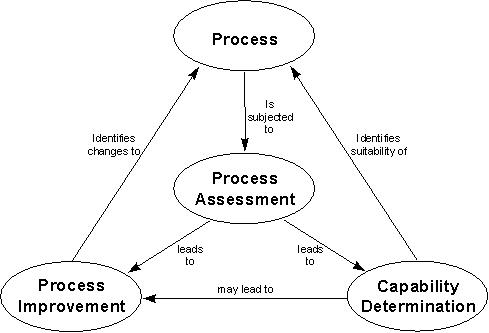
\includegraphics[scale=.6]{img/Spy.png}
		\caption{Modello SPY}
		\label{fig:ModelloSpy}
\end{figure}
\\Lo standard identifica e definisce nove attributi di qualità:
\smallskip
\begin{enumerate}
    \item \textbf{Process performance attribute}: un processo raggiunge i suoi obiettivi, trasformando input identificabili in output identificabili.
    \item \textbf{Performance management attribute}: l'attuazione di un processo è pianificata e controllata al fine di produrre risultati che rispondano agli obiettivi attesi.
    \item \textbf{Work product management attribute}: capacità del processo di elaborare un prodotto documentato, controllato e verificato.
    \item \textbf{Process definition attribute}: l'esecuzione del processo si basa su standard di processo per raggiungere i propri obiettivi;
    \item \textbf{Process resource attribute}: capacità del processo di attingere a risorse tecniche e umane appropriate per essere attuato efficacemente.
    \item \textbf{Process measurement attribute}: i risultati raggiunti e le misure rilevate durante l'attuazione di un processo sono stati usati per assicurarsi che l'attuazione di tale processo supporti efficacemente il raggiungimento di specifici obiettivi.
    \item \textbf{Process control attribute}: il processo viene controllato attraverso la raccolta, analisi ed utilizzo delle misure di prodotto e di processo, al fine di correggere, se necessario, le sue modalità di attuazione.
    \item \textbf{Process change attribute}: i cambiamenti strutturali, di gestione e di esecuzione vengono gestiti in modo controllato;
    \item \textbf{Continuous improvement attribute}: le modifiche al processo sono identificate e implementate per garantire il miglioramento continuo nella realizzazione degli obiettivi di business dell'organizzazione.
\end{enumerate}
\smallskip
La norma definisce poi quattro livelli di possesso di ciascun attributo:
\smallskip
\begin{itemize}
	\item \textbf{N} - Non posseduto (0\%-15\% di possesso): non c'è evidenza oppure ce n'è poca del possesso di un attributo.
	\item \textbf{P} - Parzialmente posseduto (16\%-50\% di possesso): vi è evidenza di approccio sistematico al raggiungimento del possesso di un attributo, ma alcuni aspetti del possesso possono essere non prevedibili;
    \item \textbf{L} - Largamente posseduto (51\%-85\% di possesso): vi è evidenza di approccio sistematico al raggiungimento di un significativo livello di possesso di un attributo, ma l'attuazione del processo può variare nelle diverse unità operative della organizzazione;
	\item \textbf{F} - (Fully) Pienamente posseduto (86\%-100\% di possesso): vi è evidenza di un approccio completo e sistematico e di un pieno raggiungimento del possesso dell'attributo, non esistono significative differenze nel modo di attuare il processo tra le diverse unità operative.
\end{itemize}
\smallskip
Vi sono infine cinque livelli di maturità di processi:
\smallskip
\begin{itemize}
	\item \textbf{Livello 0 - Processo incompleto}: il processo non è implementato o non raggiunge gli obiettivi. Non vi è evidenza di approcci sistematici agli
	attributi definiti.
	\item \textbf{Livello 1 - Processo semplicemente attuato}: il processo viene messo in atto e raggiunge i suoi obiettivi. Non vi è evidenza di un approccio sistematico ad alcuno degli attributi definiti. Il raggiungimento di questo livello è dimostrato attraverso il possesso degli attributi di ``process performance''.
	\item \textbf{Livello 2 - Processo gestito}:
	\item \textbf{Livello 3 - Processo definito}:
	\item \textbf{Livello 4 - Processo predicibile}:
	\item \textbf{Livello 5 - Processo ottimizzante}:
\end{itemize}

\subsection{Qualità del Prodotto}
\subsubsection{Funzionalità}
\subsubsection{Affidabilità}
\subsubsection{Efficienza}
\subsubsection{Usabilità}
\subsubsection{Manutenibilità}
\subsubsection{Portabilità}